\documentclass[pdftex,12pt,a4paper]{report}
\usepackage[nottoc]{tocbibind}
\setcounter{tocdepth}{4}
\setcounter{secnumdepth}{4}
\usepackage[dvipsnames]{xcolor}
\usepackage[pdftex]{graphicx}
\usepackage{float}
\usepackage{fancyvrb}
\usepackage{dtklogos}
\fvset{xleftmargin=2em}

\usepackage{pgfplots}
\pgfplotsset{width=10cm,compat=1.9}
\usepackage{tikzscale}
\usepackage{pgfplotstable}
\usepackage{booktabs}
\usepackage[font=small,labelfont=bf,tableposition=top]{caption}

\usepackage[utf8]{inputenc}
\usepackage[portuges]{babel}
\usepackage[T1]{fontenc}
\usepackage{times}
%\usepackage{lmodern}
\usepackage[obeyspaces,spaces]{url}
\usepackage[left=20mm,right=20mm,top=25mm,bottom=25mm]{geometry}
\usepackage{titlesec}
\usepackage{mathtools}
\usepackage{amsfonts}
\usepackage{hologo}
%identa 1º paragrafo de capitulos e secções
\usepackage{indentfirst}
\usepackage{url}
%\usepackage{alltt}
\usepackage[]{hyperref}
\usepackage{xspace}

\hypersetup{
%pdftitle={Trabalho 1 - Gestão de Projeto},
%pdfauthor={Bruno Pereira},
%pdfsubject={Investigação Operacional},
%pdfkeywords={keyword1, keyword2}},
bookmarksnumbered=true,     
bookmarksopen=true,         
bookmarksopenlevel=1,       
colorlinks=true,            
pdfstartview=Fit,           
pdfpagemode=UseOutlines, % this is the option you were lookin for
pdfpagelayout=TwoPageRight
		}

\usepackage{minted}
\usemintedstyle{borland}
\setminted{
%frame=lines,
%framesep=2mm,
baselinestretch=1.2,
fontsize=\footnotesize,
linenos, 
breaklines,
breakautoindent=false,
autogobble
}
\usepackage{caption}
\usepackage[final]{pdfpages}
\captionsetup[table]{aboveskip=0pt}
\captionsetup[table]{belowskip=10pt}
\usepackage{longtable}
\usepackage{subfigure}
\newenvironment{longlisting}{\captionsetup{type=listing}}{}


\usepackage{listings}

\begin{document}

\begin{titlepage}

\includepdf[pages={1}]{./report-TP2/frontTP2.pdf}
\end{titlepage}


\tableofcontents

\chapter{Parte I}

\section{Análise do problema}

O objetivo da primeira parte corresponde a modelar a gestão de inventário para a empresa fictícia W\&W, através da aplicação da política de gestão de inventários do tipo Nível de Encomenda. Esta empresa armazena o stock comprado ao fabricante no seu armazém central, que por sua vez o distribui por três lojas para venda ao público. O armazém e as lojas operam de forma diferente, facto que requere a criação de um modelo diferente para cada tipo de entidade.

\subsection{Pressupostos assumidos} 

Considerando que a falta de stock numa loja resulta na perda do lucro associado á venda do artigo, ou seja, a diferença entre o preço de venda ao cliente final e o preço de aquisição ao fabricante. Consequentemente, foi assumido que o custo de quebra nas lojas é igual á margem de lucro perdida na venda de cada artigo.

A margem de lucro em cada artigo vendido é também o custo de quebra assumido para o armazém, pois este distribui o stock da empresa pelas três lojas de venda ao público. A quebra de stock no armazém irá inevitavelmente interromper o fornecimento de artigo ás lojas, causando a perda de vendas, e do lucro associado. 

A taxa de procura para o armazém não está especificada no enunciado. No entanto, a taxa de procura diária de cada uma das três lojas cujo stock provem do armazém segue uma distribuição uniforme, entre 0 a 5 unidades. Considerando este facto, é plausível assumir que a procura diária para o armazém é igual á soma da procura nas três lojas de que o armazém fornece.  

É também conveniente considerar que os artigos comercializados por a W\&W não requerem nenhuma atenção especial do ponto de vista logístico. Num caso real, as propriedades inerentes a cada artigo podem levantar dificuldades operacionais, ou até mesmo tornar certas políticas de gestão inventário impraticáveis. 

Por fim, apesar de todas as distribuições usadas na parte I do trabalho serem uniformes, assumimos, segundo as indicações do enunciado, que todas as variáveis \emph{DDLT} seguem leis Normais. 

\newpage

\subsection{Cálculos}

Para modelar a gestão de inventário da empresa W\&W, será necessário determinar a quantidade de encomenda \emph{q}, e o nível de inventário \emph{S}. No enunciado são providenciados os seguintes dados:

\begin{itemize}
	\item \emph{Dados relativos ao armazém:}
		\begin{itemize}
			\item Valor de aquisição por artigo: 70 euros;
			\item Custo por encomenda á fábrica: 200 euros;
			\item Tempo de entrega da fábrica: 10 + (D1/2) dias;
			\item Taxa de posse anual: 21\%;
		\end{itemize}
	\item \emph{Dados relativos ás lojas:}
		\begin{itemize}
			\item Procura: Distribuição uniforme, entre 0 a 5 unidades;
			\item Preço unitário de venda: 100 euros;
			\item Custo por entrega do armazém: 2.75 euros;
			\item Tempo de entrega do armazém: 3 dias;
			\item Taxa de posse anual: 25\%;
		\end{itemize}
\end{itemize}

\subsection{Política Nível de Encomenda para o armazém}

O armazém é responsável por a gestão do nível de inventário da empresa, servindo de intermediário entre o fabricante do artigo e as lojas de venda ao público. Utilizando os dados anteriormente referidos determinamos:

\begin{itemize}
	\item Prazo de entrega \emph{l} = 10 + \frac{8}{2} = 14  dias;
	\item Custo anual de posse \emph{C1} = \emph{b} \times \emph{i} = 70 \times 0.21 = 14.70 euros por artigo por ano;
	\item Custo de quebra \emph{C2} = 100 - 70 = 30 euros por artigo;
	\item Custo de passagem de encomenda \emph{C3} = 200 euros por encomenda;
\end{itemize}

Para o cálculo do prazo de entrega de uma encomenda ao armazém, foi usado o último dígito do número de aluno 72628.

Tal como anteriormente referido, assume-se para o armazém uma procura uniformemente distribuída, entre 0 e 15 unidades, que corresponde á soma das procuras individuais de cada loja por este abastecida. Desta forma, é utilizado:

\begin{itemize}
	\item Distribuição \emph{X} \approx Uniforme[0;15];
	\item Média da distribuição: \frac{15 - 0}{2} = 7.5 unidades;
	\item Desvio padrão: \sqrt{18.75} = 4.3301;
\end{itemize}

Inicializando o processo de cálculo com \emph{E(DDLT > S)} = 0:

\begin{itemize}
	\item \emph{1ª iteração:}
	\emph{q*}=\sqrt{\frac{2 \times r \times (C2 \times E(DDLT > S) + C3)}{C1}}
	\emph{q*}=\sqrt{\frac{2 \times 7.5 \times 365 \times (30 \times 0 + 200)}{14.70}}
	\emph{q*}=272.9281 \approx 273 unidades;

	Com \emph{q} determinado, é possível calcular \emph{P(DDLT > S)} com:

	\emph{P(DDLT > S)}=\frac{\emph{C1 \times q}}{\emph{C2 \times r}}
	\emph{P(DDLT > S)}=\frac{14.70 \times 273}{30 \times 7.5 \times 365}
	\emph{P(DDLT > S)}=0.0489;

	Através da tabela \emph{Área da Distribuição Normal Standard, N(0,1)}, disponível nos apontamentos da unidade curricular, obtem-se \emph{Z} \approx 1.66;
	
	Para determinar o segundo integral, necessário ao calculo de \emph{E(DDLT > S)}, temos:
	
	\emph{Z}=\frac{3 \times \emph{N}}{100}
	\emph{N}=55;

	Através da tabela \emph{Função de Densidade Normal Standard, N(0,1)}, disponível nos apontamentos da unidade curricular, obtem-se o segundo integral: 0.018440;

	Com o segundo integral, é possível calcular \emph{E(DDLT > S)}, utilizando:

	\emph{E(DDLT > S)} = \emph{segundo integral} \times \emph{\sigma}\emph{DDLT}
	\emph{E(DDLT > S)} = 0.018440 \times \sqrt{emph{l} \times \emph{sigma_r^2}}
	\emph{E(DDLT > S)} = 0.018440 \times \sqrt{14 \times 4.3301}
	\emph{E(DDLT > S)} = 0.018440 \times 7.7860
	\emph{E(DDLT > S)} = 0.1436;

	\emph{S} = \emph{\mu}\emph{DDLT} + \emph{Z} \times \emph{\sigma}\emph{DDLT}
	\emph{S} = \emph{r} \times \emph{l} + \emph{Z} \times \emph{\sigma}\emph{DDLT}
	\emph{S} = 7.5 \times 14 + 1.66 \times 7.7860
	\emph{S} = 117.9248 \approx 118 unidades;

	
\item \emph{2ª iteração:}
	
	Para a segunda iteração é utilizado \emph{E(DDLT > S)} = 0.1436;
	
	\emph{q*}=\sqrt{\frac{2 \times r \times (C2 \times E(DDLT > S) + C3)}{C1}}
	\emph{q*}=\sqrt{\frac{2 \times 7.5 \times 365 \times (30 \times 0.1436 + 200)}{14.70}}
	\emph{q*}=275.8519 \approx 276 unidades;

	Com \emph{q} determinado, é possível calcular \emph{P(DDLT > S)} utilizando:

	\emph{P(DDLT > S)}=\frac{\emph{C1 \times q}}{\emph{C2 \times r}}
	\emph{P(DDLT > S)}=\frac{14.70 \times 276}{30 \times 7.5 \times 365}
	\emph{P(DDLT > S)}=0.0494;

	Através da tabela \emph{Área da Distribuição Normal Standard, N(0,1)}, disponível nos apontamentos da unidade curricular, obtem-se \emph{Z} \approx 1.65;
	
	Para determinar o segundo integral, necessário ao calculo de \emph{E(DDLT > S)}, temos:
	
	\emph{Z}=\frac{3 \times \emph{N}}{100}
	\emph{N}=55;

	Através da tabela \emph{Função de Densidade Normal Standard, N(0,1)}, disponível nos apontamentos da unidade curricular, obtem-se o segundo integral: 0.018440;

	Com o segundo integral, é possível calcular \emph{E(DDLT > S)}, com:

	\emph{E(DDLT > S)} = 0.018440 \times \emph{\sigma}\emph{DDLT}
	\emph{E(DDLT > S)} = 0.018440 \times \sqrt{emph{l} \times \emph{sigma_r^2}}
	\emph{E(DDLT > S)} = 0.018440 \times \sqrt{14 \times 4.3301}
	\emph{E(DDLT > S)} = 0.018440 \times 7.7860
	\emph{E(DDLT > S)} = 0.1436;

	Como o valor de \emph{E(DDLT > S)} da iteração atual é igual ao valor da iteração anterior, esta é a última iteração.

	\emph{S} = \emph{\mu}\emph{DDLT} + \emph{Z} \times \emph{\sigma}\emph{DDLT}
	\emph{S} = \emph{r} \times \emph{l} + \emph{Z} \times \emph{\sigma}\emph{DDLT}
	\emph{S} = 7.5 \times 14 + 1.65 \times 7.7860
	\emph{S} = 117.8469 \approx 118 unidades;

\end{itemize}

De acordo com os cálculos efetudos, determinamos para o armazém os seguintes valores:

\begin{itemize}
\item Quantidade de encomenda \emph{q}: 276 unidades;
\item Nível de inventário \emph{S}: 118 unidades;
\end{itemize}

Os resultados obtidos permitem concluir que uma ordem de encomenda com a quantia constante de 276 unidades deverá ser enviada sempre que o stock em armazém atinge valores inferiores a 118 artigos. Adicionalmente, e sendo a procura conhecida, é possível calcular o valor aproximado de:

\begin{itemize}
\item Frequência de encomendas: \frac{\emph{q}}{\emph{r}} = \frac{276}{7.5} \approx 37 dias;
\item Encomendas anuais: \frac{\emph{r}}{\emph{q}} = \frac{7.5 \times 365}{276} \approx 10 encomendas;
\end{itemize}

Ao seguir esta política, o armazém realizará por ano cerca de 10 encomendas, com um intervalo entre dois pedidos de encomenda consecutivos aproximadamente igual a 37 dias.   


\subsection{Política Nível de Encomenda para as lojas}

Para cada uma das lojas, são especificados os seguintes dados:

\begin{itemize}
\item Custo anual de posse \emph{C1} = \emph{b} \times \emph{i} = 70 \times 0.25 = 17.50 euros por artigo por ano;
\item Custo de quebra \emph{C2} = 30 euros por artigo;
\item Custo de passagem de encomenda \emph{C3} = 2.75 euros por encomenda;
\item Procura 
\end{itemize}

A procura em cada uma das lojas segue uma distribuição uniforme, entre 0 a 5 unidades de artigo. Consequentemente, temos:

\begin{itemize}
\item Distribuição \emph{X} \approx Uniforme[0;5];
\item Média da distribuição: \frac{5 - 0}{2} = 2.5 unidades
\item Variância: \frac{(5 - 0)^2}{12} = 2.0833;
\item Desvio padrão: \sqrt{2.0833} = 1.4434;
\end{itemize}

Inicializando o processo de cálculo com \emph{E(DDLT > S)} = 0:

\begin{itemize}
\item \emph{1ª iteração:}

	\emph{q*}=\sqrt{\frac{2 \times r \times (C2 \times E(DDLT > S) + C3)}{C1}}
	\emph{q*}=\sqrt{\frac{2 \times 2.5 \times 365 \times (30 \times 0 + 2.75)}{17.50}}
	\emph{q*}=16.9347 \approx 17 unidades;

	Com \emph{q} determinado, é possível calcular \emph{P(DDLT > S)} utilizando:

	\emph{P(DDLT > S)}=\frac{\emph{C1 \times q}}{\emph{C1 \times q}+\emph{C2 \times r}}
	\emph{P(DDLT > S)}=\frac{\emph{17.50 \times 17}}{\emph{17.50 \times 17}+\emph{30 \times 2.5 \times 365}}
	\emph{P(DDLT > S)}=0.0108;

	Utilizando o valor de \emph{P(DDLT > S)}, é possível determinar \emph{S} com:
	
	\emph{P(DDLT > S)}=\int_S^5 \mathrm{p(n)}\,\mathrm{d}x
	0.0108=\int_S^5 \mathrm{1/5}\,\mathrm{d}x
	0.0108=\dfrac{5}{5} - \dfarc{S}{5}
	\emph{S}=4.946 unidades;

	Com \emph{S} calculado, determinamos \emph{E(DDLT > S)} utilizando:
	
	\emph{E(DDLT > S)}=\int_S^5 \mathrm{xp(n)}\,\mathrm{d}x - emph{S} \times \emph{P(DDLT > S)}
	\emph{E(DDLT > S)}=\frac{25}{10} - \frac{24.4630}{10} - 4.946 \times 0.0108
	\emph{E(DDLT > S)} = 0.0003;


\item \emph{2ª iteração:}
	
	Para a segunda iteração é utilizado \emph{E(DDLT > S)} = 0.0003;

	\emph{q*}=\sqrt{\frac{2 \times r \times (C2 \times E(DDLT > S) + C3)}{C1}}
	\emph{q*}=\sqrt{\frac{2 \times 2.5 \times 365 \times (30 \times 0.0003 + 2.75)}{17.50}}
	\emph{q*}=16.9624 \approx 17 unidades

	Com \emph{q} determinado, é possível calcular \emph{P(DDLT > S)} utilizando:

	\emph{P(DDLT > S)}=\frac{\emph{C1 \times q}}{\emph{C1 \times q}+\emph{C2 \times r}}
	\emph{P(DDLT > S)}=\frac{\emph{17.50 \times 17}}{\emph{17.50 \times 17}+\emph{30 \times 2.5 \times 365}}
	\emph{P(DDLT > S)}=0.0108;

	Utilizando o valor de \emph{P(DDLT > S)}, é possível determinar \emph{S} com:
	
	\emph{P(DDLT > S)}=\int_S^5 \mathrm{p(n)}\,\mathrm{d}x
	0.0108=\int_S^5 \mathrm{1/5}\,\mathrm{d}x
	0.0108=\frac{5}{5} - \farc{S}{5}
	\emph{S}=4.946 unidades;

	Com \emph{S} calculado, determinamos \emph{E(DDLT > S)} utilizando:
	
	\emph{E(DDLT > S)}=\int_S^5 \mathrm{xp(n)}\,\mathrm{d}x - emph{S} \times \emph{P(DDLT > S)}
	\emph{E(DDLT > S)}=\frac{25}{10} - \frac{24.4630}{10} - 4.946 \times 0.0108
	\emph{E(DDLT > S)} = 0.0003;

	O valor de \emph{E(DDLT > S)} da interação atual é igual ao valor da iteração anterior, logo, esta é a última iteração.

\end{itemize}

De acordo com os cálculos efetudos, determinamos para cada uma das lojas os seguintes valores:

\begin{itemize}
\item Quantidade de encomenda \emph{q}: 17 unidades;
\item Nível de inventário \emph{S}: 5 unidades;
\end{itemize}

Os resultados obtidos permitem concluir que uma ordem de reabastecimento com a quantia constante de 17 unidades deverá ser enviada sempre que o stock em loja atinge valores inferiores a 5 artigos. Adicionalmente, e sendo a procura conhecida, é possível calcular o valor aproximado de:

\begin{itemize}
\item Frequência de encomendas: \frac{\emph{q}}{\emph{r}} = \frac{17}{2.5} \approx 7 dias;
\item Encomendas anuais: \frac{\emph{r}}{\emph{q}} = \frac{2.5 \times 365}{17} \approx 54 encomendas;
\end{itemize}

Ao seguir esta política, cada loja lançará por ano cerca de 54 pedidos de reabastecimento, com um intervalo entre dois pedidos consecutivos aproximadamente igual a 7 dias.   




\chapter{Parte II}

\section{Análise do problema}

Na segunda parte é proposto ao grupo simular a gestão da empresa W\&W por um período de 200 dias, recorrendo ao software "Jogo da DIstribuição", facultado com o enunciado do trabalho. O objetivo será maximizar o lucro total durante o período especificado, utilizando a política de encomenda determinada na parte anterior.

\section{Resultados obtidos}

\subsection{Nível de stock}

As seguintes tabelas apresentam a evolução do nível de stock a cada 40 dias de operação: 

\begin{table}[htpb]
\begin{center}
\begin{tabular}{cc}
\toprule
Dia & Stock	 	\\ \midrule
40 & 146                \\ 
80 & 116                \\ 
120 & 103               \\ 
160 & 107               \\ 
200 & 77     		\\ 
\bottomrule
\end{tabular}
\end{center}
\caption{Nível de stock no armazém}
\label{tab:tabela1}
\end{table}



\begin{table}[htpb]
\begin{center}
\begin{tabular}{cc}
\toprule
Dia & Stock	 	\\ \midrule
40 & 12                 \\ 
80 & 17                 \\ 
120 & 8                 \\ 
160 & 10                \\ 
200 & 25     		\\ 
\bottomrule
\end{tabular}
\end{center}
\caption{Nível de stock na loja 1}
\label{tab:tabela2}
\end{table}



\begin{table}[htpb]
\begin{center}
\begin{tabular}{cc}
\toprule
Dia & Stock	       \\ \midrule
40 & 6                 \\ 
80 & 1                 \\ 
120 & 13               \\ 
160 & 30               \\ 
200 & 16     	       \\ 
\bottomrule
\end{tabular}
\end{center}
\caption{Nível de stock na loja 2}
\label{tab:tabela3}
\end{table}



\begin{table}[htpb]
\begin{center}
\begin{tabular}{cc}
\toprule
Dia & Stock	 	\\ \midrule
40 & 17                 \\ 
80 & 16                 \\ 
120 & 6                 \\ 
160 & 14                \\ 
200 & 9     		\\ 
\bottomrule
\end{tabular}
\end{center}
\caption{Nível de stock na loja 3}
\label{tab:tabela4}
\end{table}




\subsection{Saldo Acumulado}

No gráfico abaixo está representada a evoulução do saldo acumulado durante os 200 dias de jogo:

\begin{figure}[<+htpb+>]
	\centering
	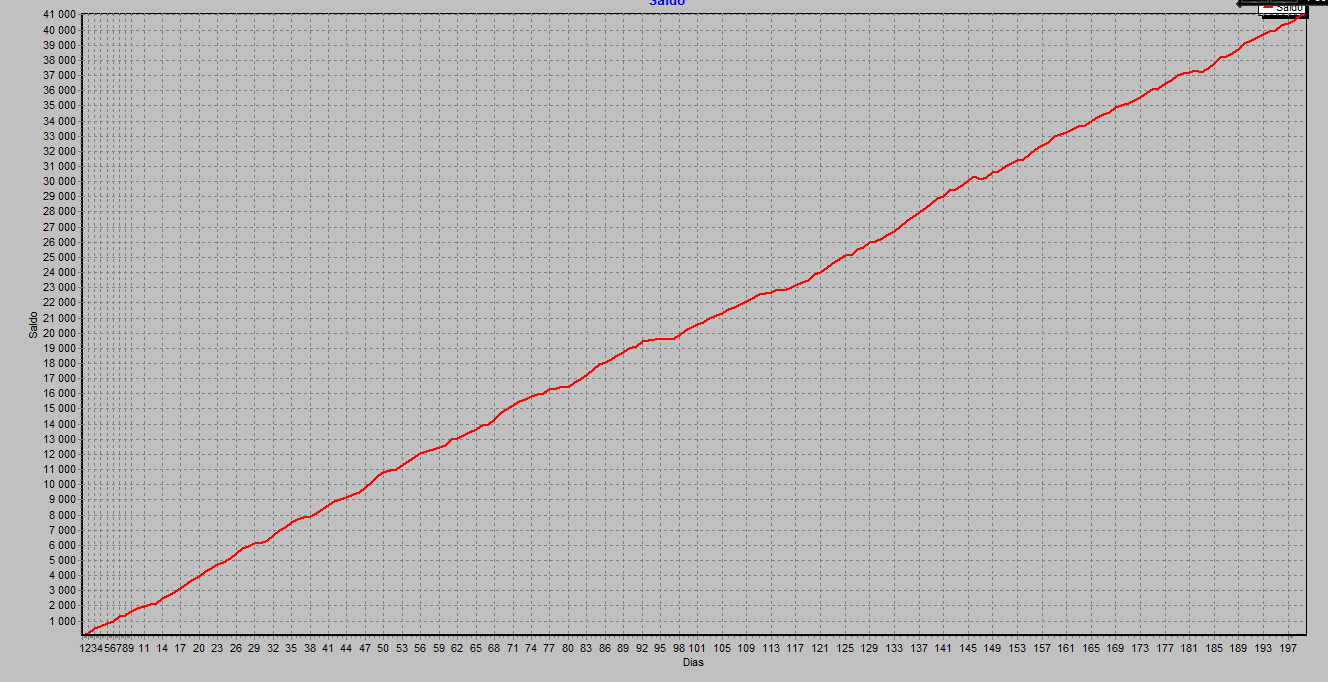
\includegraphics[scale=0.75]{./report-TP2/img/saldo.png}
	\caption{Saldo acumulado no final do jogo}
\label{fig:figure1}
\end{figure}



\subsection{Estratégia de jogo}

No dia inicial o stock do armazém foi inicializado em 125 unidades, e o stock de cada uma das lojas a 25 unidades. A política de encomendas seguida tanto para as lojas como para o armazém corresponde á política determinada na parte I para cada entidade:

\begin{itemize}
	\iteam \emph{Política de encomendas para o armazém}
		\begin{itemize}
			\item \emph{q} = 276 unidades;
			\item \emph{S} = 118 unidades;
			\item Frequência de encomenda: 37 dias;
		\end{itemize}
	\iteam \emph{Política de encomendas para as lojas}
		\begin{itemize}
			\item \emph{q} = 17 unidades;
			\item \emph{S} = 5 unidades;
			\item Frequência de encomenda: 7 dias;
		\end{itemize}
\end{itemize}

A política de Nível de encomenda foi seguida á risca durante o jogo. Tanto para o armazém como para as lojas, sempre que o nível de inventário descia abaixo de \emph{S}, ou o número de dias desde o último pedido igualava o valor de frequência de encomenda, era simulada a encomenda de \emph{q} unidades de artigo para a entidade correspondente. Terminados os 200 dias, foi obtido um saldo final de aproximadamente 40705 euros.





\appendix

\part*{ANEXOS}
\addcontentsline{toc}{part}{ANEXOS}
\refstepcounter{part} 

\chapter{A}

\subsection{Evolução do nível de inventário durante o período de jogo}

\begin{figure}[<+htpb+>]
	\centering
	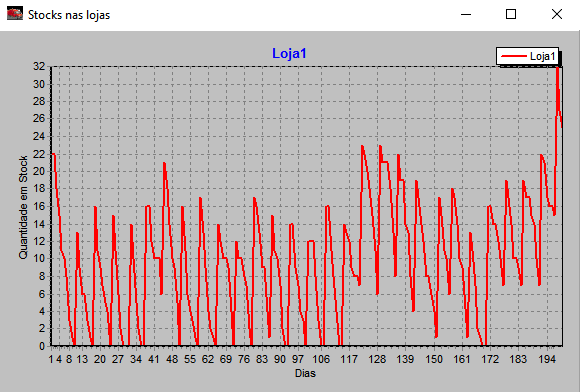
\includegraphics[scale=0.75]{./report-TP2/img/loja1.png}
	\caption{Evoulução do nível de inventário na loja 1}
\label{fig:figure2}
\end{figure}


\begin{figure}[<+htpb+>]
	\centering
	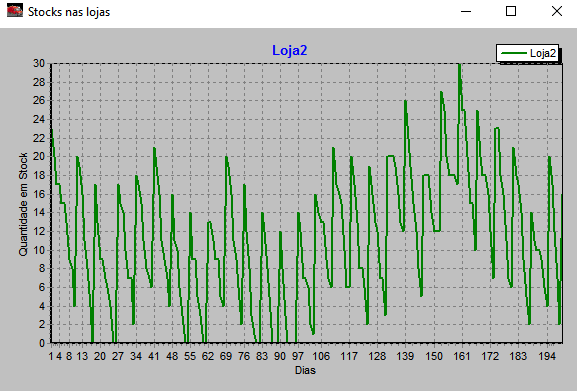
\includegraphics[scale=0.75]{./report-TP2/img/loja2.png}
	\caption{Evoulução do nível de inventário na loja 2}
\label{fig:figure3}
\end{figure}


\begin{figure}[<+htpb+>]
	\centering
	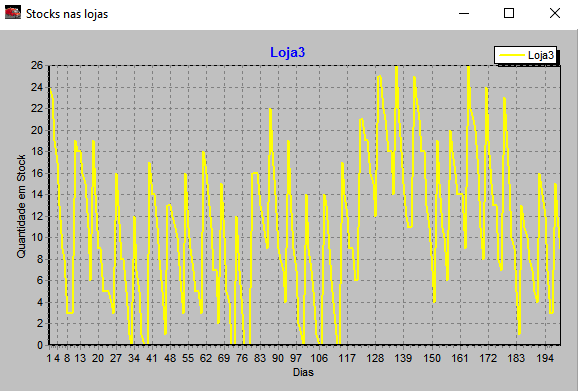
\includegraphics[scale=0.75]{./report-TP2/img/loja3.png}
	\caption{Evoulução do nível de inventário na loja 3}
\label{fig:figure4}
\end{figure}


\input{./report-TP2/fig/figuraLojaArmazem}


\end {document}


